\documentclass[10pt,twocolumn]{article}

\usepackage[a4paper, top=30mm, bottom=20mm, left=10mm, right=10mm]{geometry}
\usepackage[hangul]{kotex}
\newcommand{\titleko}{람다 대수를 응용한 자연 연역 체계의 전산화에 관한 연구}
\newcommand{\titleen}{Computerizing natural deduction using lambda calculus}
\newcommand{\authorname}{이상길}
\newcommand{\getkeywords}{수학기초론, 람다 대수, 형식 체계}
\usepackage[pdfencoding=unicode,
	pdfauthor={\authorname},
	pdftitle={\titleko},
	pdfkeywords={\getkeywords},
	bookmarks]{hyperref}
\usepackage{amsmath, amscd, amsthm, amssymb, amsfonts, mathrsfs, mathtools, mathalfa}
\usepackage{abstract}
\usepackage[sans]{dsfont}
\usepackage{latexsym}
\usepackage{enumitem}
\usepackage{color}
\usepackage{url}
\usepackage{graphicx}
\graphicspath{{./images/}}
\usepackage{multirow}
\usepackage{float}
\usepackage{listings}
\usepackage[square,numbers]{natbib}
\bibliographystyle{ieeetr}
\usepackage{caption}
\captionsetup[table]{skip=.5em}
\usepackage{fitch}
\usepackage{bm}
\usepackage{adjustbox}

\definecolor{javared}{rgb}{0.6,0,0}
\definecolor{javapurple}{rgb}{0.5,0,0.35}

\lstdefinelanguage{mom}{
	keywords={type,axiom,theorem},
	sensitive=true,
	keywordstyle=\color{javapurple}\ttfamily,
	morecomment=[s][\color{javared}]{<}{>},
}

\lstset{
	language=mom,
	basicstyle=\small\ttfamily,
	tabsize=4
}

\theoremstyle{definition}
\newtheorem{theorem}{정리}
\newtheorem{definition}[theorem]{정의}
\newtheorem{example}[theorem]{예시}

\newcommand{\N}{\mathbb{N}}
\newcommand{\Z}{\mathbb{Z}}
\newcommand{\Q}{\mathbb{Q}}
\newcommand{\R}{\mathbb{R}}

\newcommand{\sinc}{\operatorname{sinc}}
\newcommand{\dom}{\operatorname{dom}}
\newcommand{\im}{\operatorname{im}}
\newcommand{\ord}{\operatorname{ord}}
\newcommand{\Prop}{\mathsf{Prop}}
\newcommand{\Set}{\mathsf{Set}}
\newcommand{\Cls}{\mathsf{Cls}}
\newcommand{\leqnormal}{\mathrel{\unlhd}}
\newcommand{\ltnormal}{\mathrel{\lhd}}

\newcommand{\lch}{\bm\lambda_\to^{\text{Ch}}}
\newcommand{\lchh}{\bm\lambda_{\to,\vdash}^{\text{Ch}}}
\newcommand{\Lch}{\Lambda_\to^{\text{Ch}}}
\newcommand{\Lchh}{\Lambda_{\to,\vdash}^{\text{Ch}}}

\newcommand{\fv}{\mathbf{FV}}
\newcommand{\bv}{\mathbf{BV}}

% \renewcommand{\abstractname}{초 록}
\renewcommand{\refname}{참고문헌}
\kscntformat{section}{}{}

\title{\titleko\\[1ex]\large\titleen}
\author{\authorname\thanks{\href{mailto:ossia@korea.ac.kr}{\texttt{ossia@korea.ac.kr}}}}
\date{}

\begin{document}

\twocolumn[
\begin{@twocolumnfalse}
	\maketitle
	\begin{abstract}
		\centering\begin{minipage}{\dimexpr\paperwidth-8cm}
			\noindent 이 논문에서는 형식 체계를 만들고, 만들어진 형식 체계에서 컴퓨터에 의해 검증되는 증명을 할 수 있도록 하는 컴퓨터 프로그램을 만드는 방법에 관하여 연구한다. 이를 위하여 람다 대수를 기반으로 형식 언어를 만들며 가언적 추론을 지원하는 형식 체계를 만들었으며 컴퓨터 프로그램도 만들었다. 재미난 추론 규칙들을 갖는다. 재미난 정리들도 증명했다.
			
			\smallskip\noindent {\bf 주제어}: \getkeywords
		\end{minipage}
	\end{abstract}\vspace{2em}
\end{@twocolumnfalse}
]

\saythanks

\section{서론}

람다 대수의 타입 체계와 자연 연역 체계 간에 대응 관계가 있음은 잘 알려져 있다\cite{howard}.

형식 체계를 전산화하는 것은 필요하다. Metamath나 Coq 같은 것이 이미 있다. Metamath는 가언적 추론(假言的推論, hypothetical derivation)을 지원하지 않고 Coq은 Curry--Howard 동치에 기반한다. 우리 체계는 Curry--Howard 동치에 의존하지 않으며 함수 타입이 논리적 $\to$에 대응된다고 생각하지 않는다.

\section{형식 언어의 정의}

형식 체계가 성립하기 위하여는 먼저 형식 체계가 사용할 언어가 구축되어야 한다. 우리의 체계에서 언어 상의 모든 문장은 타입을 갖도록 할 것인데, 예를 들어 ``$1+1=2$''와 같은 명제는 명제 타입 $\Prop$을 가질 것이고, 연언(連言)을 뜻하는 이항연산자 $\land$는 두 개의 명제를 받아 새로운 명제를 만드는 함수이므로 $\Prop\times\Prop\to\Prop$ 타입을 가질 것이다. 이때 $p$ 및 $q$가 명제인 경우 $p\land q$는 이항연산자 $\land$에 인자 $(p, q)$를 주어 호출한 것이며 $p\land q$의 타입은 $\land$의 반환 타입인 $\Prop$이 된다. 예시로부터 알 수 있듯 우리의 언어는 함수의 생성이나 호출에 관한 구문을 지원하여야 하며, 즉 우리의 언어는 특정 조건을 만족하는 람다 항의 집합이 되어야 한다.

또한 우리의 언어는 추론 규칙(rule of inference)에 대한 표현력을 가질 것이다. 예를 들어 Hilbert 체계에서 추론 규칙 중 하나인 전건 긍정(modus ponens) $p, p\to q\vdash q$는 메타문장이며 논리식의 언어에 속하지 않지만 우리의 체계는 이를 언어에 포함시킬 것이다. 또 우리 체계는 문장
$$p_1,p_2,\ldots,p_n\text{\ \ 및\ \ }p_1, p_2, \ldots, p_n\vdash q$$
로부터 $q$를 유도할 수 있도록 하는 추론 규칙을 가질 것이다. 이는 예를 들어
$$p\text{\ \ 및\ \ }p\to q\text{\ \ 및\ \ }p, p\to q\vdash q$$
로부터 $q$를 유도할 수 있도록 한다. 이러한 방식을 적용하면 일반적으로 추론 규칙인 것들이 우리의 형식 체계에서 공리로 표현되게 되며, 우리의 형식 체계는 체계 내부에서 다른 형식 체계의 동작을 모사할 수 있게 된다. 이는 우리의 체계를 사용하는 자가 체계 내부에 자신만의 형식 체계를 만들 수 있도록 하며, 단순히 공리계를 만들 수 있도록 하는 것보다 더 많은 자유를 부여한다.

그러므로 우리의 언어를 구성하기 위해서는 단순 타입 람다 대수(simply typed lambda calculus)에 $\vdash$ 구문을 추가할 필요가 있다. $\lch$가 \cite{luswt}의 정의~1.1.30과 같이 정의된다고 하자. $\lch$에서는 모든 변항(變項)에 고유한 타입이 지정되어 있어서 타이핑 문맥(typing context)이 필요하지 않다. 이제 $\lch$에 $\vdash$ 구문을 추가하여 새로운 체계 $\lchh$를 만들어 보자. 먼저 타입 생성자 $\vdash$를 추가하기 위하여 \cite{luswt}의 정의~1.1.11의 BNF를 다음과 같이 수정하자.
$$\mathds T \Coloneqq \mathbb A\mid\mathds T\to\mathds T\mid\mathds T\vdash\mathds T.$$
또 $M\vdash N$ 형태의 람다 항이 생성될 수 있도록 \cite{luswt}의 정의~1.1.30(ii)에 다음과 같은 규칙을 추가하자.
$$M\in\Lchh(A), N\in\Lchh(B)\Rightarrow (M\vdash N)\in\Lchh(A\vdash B).$$
또 우리 체계는 함수의 외연성(extensionality)을 받아들여 $\bm{\lambda\beta\eta}$를 equational theory로 사용할 것인데, $\bm{\lambda\beta\eta}$에 $\vdash$에 대한 합동 규칙
$$\dfrac{M=M'\quad N=N'}{(M\vdash N)=(M'\vdash N')}$$
을 추가하여야 한다. 이때 Church식 의미론에 의하여 $A\ne B$일 때 $\lambda x^A.x^A\ne\lambda x^B.x^B$이다.

또 $\land$나 $\forall$ 등의 무정의용어를 도입하기 위해서는 정항(正項)을 추가할 수 있어야 하는데, 정항의 집합 $\mathcal C$는 \cite{luswt}의 정의~1.1.30(i)에서 정의된 변항의 집합 $\mathsf V^{\mathds T}$의 부분집합으로 정의하자. 이때 우리의 형식 언어 $\mathcal L$은 다음과 같이 정의된다.

\begin{definition}(형식 언어)
	$\mathbb A$가 원시 타입의 집합이고 $\mathds T$가 $\lchh$ 상에서 $\mathbb A$로부터 생성된 타입의 집합일 때, 정항의 집합 $\mathcal C\subseteq \mathsf V^{\mathds T}$에 대하여 형식 언어 $\mathcal L$이 다음과 같이 정의된다.
	$$\mathcal L = \{M\in\Lchh: \mathrm{FV}(M)\subseteq\mathcal C\}.$$
\end{definition}

즉 $\mathcal L$은 $\Lchh$에 있는 람다 항 중에서 자유 변항이 전부 정항인 것들의 집합이다. 예를 들어 $\mathbb A = \{\Prop\}$이고 $$\mathcal C = \{\land^{\Prop\to\Prop\to\Prop}, \top^{\Prop}\}$$일 때 $p$가 $\Prop$ 타입이라면 $\lambda p.{\land}p\top\in\mathcal L$이고 ${\land}p\top\notin\mathcal L$이다.

\section{공리 및 추론 규칙의 정의}

우리의 형식 체계는 형식 체계의 동작을 모사하는 5개의 추론 규칙을 가진다. 가정의 집합 $\mathcal H\subseteq\Lchh$ 및 $\varphi\in\Lchh$에 대해 $\mathcal H\vdash\varphi$가 ``$\mathcal H$로부터 $\varphi$를 증명할 수 있다"는 뜻이라 하자. $\mathcal H\vdash\varphi$는 다음과 같은 공리 및 추론 규칙을 사용하여 유도할 수 있다.

\begin{definition}[공리 및 추론 규칙]
	우리 형식 체계의 공리 및 추론 규칙은 다음과 같다.
	
	\begin{enumerate}
		\item (R 규칙)\quad 임의의 $\varphi\in\mathcal H$에 대하여 $\mathcal H\vdash\varphi.$
		\item ($\mapsto$I 규칙)\quad 임의의 $\psi\in\mathcal H$에 대해 $x^A\notin\mathrm{FV}(\psi)$일 때 $$\dfrac{\mathcal H\vdash\varphi}{\mathcal H\vdash\lambda x^A.\varphi}.$$
		\item ($\mapsto$E 규칙)\quad $\varphi\psi\in\Lchh$일 때 $$\dfrac{\mathcal H\vdash\varphi}{\mathcal H\vdash\varphi\psi}.$$
		\item ($\vdash$I 규칙)\quad $\dfrac{\mathcal H\cup\{\varphi\}\vdash\psi}{\mathcal H\vdash(\varphi\vdash\psi)}.$
		\item ($\vdash$E 규칙)\quad $\dfrac{\mathcal H\vdash\varphi\quad\mathcal H\vdash(\varphi\vdash\psi)}{\mathcal H\vdash\psi}.$
	\end{enumerate}
\end{definition}

$\mathcal H\vdash\phi$의 $\vdash$와 $\varphi\vdash\psi$의 $\vdash$는 다른 기호임에 주의하라. 공리 및 추론 규칙을 $\mathcal H\vdash\varphi$ 형태의 식에 적용하는 것은 우리 체계가 가언적 추론을 지원하는 자연 연역 체계이기 때문이다.

\begin{example} \label{example:proof}
	$$\mathcal H = \left\{\begin{array}{l}
		\lambda p^\Prop\lambda q^\Prop.(p\vdash(q\vdash {\land}pq)),\\
		\lambda p^\Prop\lambda q^\Prop.({\land}pq\vdash p),\\
		\lambda p^\Prop\lambda q^\Prop.({\land}pq\vdash q)
	\end{array}\right\}$$
	일 때 위의 공리 및 추론 규칙으로부터 $$\mathcal H\vdash \lambda p^\Prop\lambda q^\Prop.({\land}pq\vdash{\land}qp)$$는 다음과 같이 증명할 수 있다.
	
	\begin{table}[H] \centering\small
		\begin{tabular}{lll}
			1 & $\mathcal H\cup\{{\land}p'q'\}\vdash {\land}p'q'$ & R \\
			2 & $\mathcal H\cup\{{\land}p'q'\}\vdash \lambda p\lambda q.({\land}pq\vdash p)$ & R \\
			3 & $\mathcal H\cup\{{\land}p'q'\}\vdash \lambda q.({\land}p'q\vdash p')$ & $\mapsto$E (2) \\
			4 & $\mathcal H\cup\{{\land}p'q'\}\vdash ({\land}p'q'\vdash p')$ & $\mapsto$E (3) \\
			5 & $\mathcal H\cup\{{\land}p'q'\}\vdash p'$ & $\vdash$E (1, 4) \\
			6 & $\mathcal H\cup\{{\land}p'q'\}\vdash \lambda p\lambda q.({\land}pq\vdash q)$ & R \\
			7 & $\mathcal H\cup\{{\land}p'q'\}\vdash \lambda q.({\land}p'q\vdash q)$ & $\mapsto$E (6) \\
			8 & $\mathcal H\cup\{{\land}p'q'\}\vdash ({\land}p'q'\vdash q')$ & $\mapsto$E (7) \\
			9 & $\mathcal H\cup\{{\land}p'q'\}\vdash q'$ & $\vdash$E (1, 8) \\
			10 & $\mathcal H\cup\{{\land}p'q'\}\vdash \lambda p\lambda q.(p\vdash (q\vdash{\land}pq))$ & R \\
			11 & $\mathcal H\cup\{{\land}p'q'\}\vdash \lambda q.(q'\vdash(q\vdash{\land}q'q))$ & $\mapsto$E (10) \\
			12 & $\mathcal H\cup\{{\land}p'q'\}\vdash (q'\vdash(p'\vdash{\land}q'p'))$ & $\mapsto$E (11) \\
			13 & $\mathcal H\cup\{{\land}p'q'\}\vdash (p'\vdash{\land}q'p')$ & $\vdash$E (9, 12) \\
			14 & $\mathcal H\cup\{{\land}p'q'\}\vdash {\land}q'p'$ & $\vdash$E (5, 13) \\
			15 & $\mathcal H\vdash ({\land}p'q'\vdash {\land}q'p')$ & $\vdash$I (14) \\
			16 & $\mathcal H\vdash \lambda q'.({\land}p'q'\vdash {\land}q'p')$ & $\mapsto$I (15) \\
			17 & $\mathcal H\vdash \lambda p'\lambda q'.({\land}p'q'\vdash {\land}q'p')$ & $\mapsto$I (16) \\
		\end{tabular}
	\end{table}
	
	그러나 위 증명은 Fitch 다이어그램으로 다음과 같이 더 간단히 표현할 수 있다.
	
	\begin{figure}[H] \centering\small
		$\begin{nd}\close
			\open[p]
			\open[q]
			\open
			\hypo{}{{\land}pq} \by{가정}{}
			\have{}{\lambda p\lambda q.({\land}pq\vdash p)} \by{R}{}
			\have{}{{\land}pq\vdash p} \by{$\mapsto$E (2)}{}
			\have{}{p} \by{$\vdash$E (1, 3)}{}
			\have{}{\lambda p\lambda q.({\land}pq\vdash q)} \by{R}{}
			\have{}{{\land}pq\vdash q} \by{$\mapsto$E (5)}{}
			\have{}{q} \by{$\vdash$E (1, 6)}{}
			\have{}{\lambda p\lambda q.(p\vdash (q\vdash{\land}pq))} \by{R}{}
			\have{}{q\vdash(p\vdash{\land}qp)} \by{$\mapsto$E (8)}{}
			\have{}{{\land}qp} \by{$\vdash$E (7, 4, 9)}{}
			\close
			\have{}{{\land}pq\vdash {\land}qp} \by{$\vdash$I (1--10)}{}
			\close
			\close
			\have{}{\lambda p\lambda q.({\land}pq\vdash {\land}qp)} \by{$\mapsto$I (1--11)}{}
		\end{nd}$
	\end{figure}
	
	단 위의 Fitch 다이어그램에서 연속된 $\mapsto$E 또는 $\vdash$E, $\mapsto$I는 하나로 표현되었다.
\end{example}

\section{형식 체계의 정의}

형식 체계는 원시 타입의 집합 $\mathbb A$, 정항의 집합 $\mathcal C\subseteq\mathsf V^{\mathds T}$, 최초 가정(``공리")의 집합 $\mathcal H_0\subseteq\mathcal L$에 의해 결정되며 이들은 우리 체계를 사용하는 자가 정할 수 있다. 이때 어떤 명제 $\varphi\in\mathcal L$이 증명 가능하다는 것은 다음과 같은 뜻이다.

\begin{definition}[증명 가능성]
	$\langle\mathbb A,\mathcal C,\mathcal H_0\rangle$에 의하여 결정되는 형식 체계에서 $\varphi\in\mathcal L$이 증명 가능하다는 것은 $\mathcal H_0\vdash\varphi$가 유도 가능하다는 뜻이다.
\end{definition}

이제부터는 함수 타입 및 $\vdash$ 타입을 언커링(uncurrying) 하여 표시하자. 예를 들어 $fxy$ 대신 $f(x, y)$라 쓰고 $p\vdash(q\vdash r)$ 대신 $p, q\vdash r$이라 쓰는 것이다. $\land$ 등의 이항연산자의 경우 ${\land}(p, q)$ 대신 $p\land q$라고도 쓸 수 있다. 또 $\lambda x^A\ldots\lambda z^C.M$ 대신 $(x^A, \ldots, z^C)\mapsto M$이라 쓰자.

\begin{example}\label{example:system}
	명제논리를 위한 형식 체계는 다음과 같이 정의해 볼 수 있다.
	
	\begin{align*}
		\mathbb A &= \{\mathsf{Prop}\}, \\
		\mathcal C &= \{\to, \neg, \land, \top\}, \\
		\mathcal H_0 &= \left\{\begin{array}{l l}
			\mathsf{cp}: & (p^\Prop, q^\Prop)\mapsto(p\vdash q)\vdash p\to q, \\
			\mathsf{mp}: & (p^\Prop, q^\Prop)\mapsto p, p\to q\vdash q, \\
			\mathsf{Ai}: & (p^\Prop, q^\Prop)\mapsto p, q\vdash p\land q, \\
			\mathsf{Ae1}: & (p^\Prop, q^\Prop)\mapsto p\land q\vdash p, \\
			\mathsf{Ae2}: & (p^\Prop, q^\Prop)\mapsto p\land q\vdash q, \\
			\mathsf{Ti}: & \top \\
			\mathsf{luk3}: & (p^\Prop, q^\Prop)\mapsto \neg p\to\neg q\vdash q\to p
		\end{array}\right\}
	\end{align*}

	$\mathcal H_0$의 각 원소 앞에 써 놓은 것은 원소들의 이름이다.
\end{example}

\subsection{매크로의 정의}

예시~\ref{example:system}의 체계에는 $\lor$, $\leftrightarrow$ 연산자 및 $\bot$도 정의되어 있는데 이들은 무정의용어로서가 아닌 다른 개념에 의존하는 매크로로서 정의되어 있으므로 무정의용어의 집합인 $\mathcal C$에 나타나지 않는다. 이들은 다음과 같이 정의되어 있다.
\begin{align*}
	\lor&\coloneqq (p^\Prop, q^\Prop)\mapsto \neg p\to q, \\
	\leftrightarrow&\coloneqq (p^\Prop, q^\Prop)\mapsto (p\to q)\land(q\to p), \\
	\bot&\coloneqq\neg\top.
\end{align*}
또 ZFC 집합론에서 단항 술어는 집합 하나를 받아 명제를 출력하는 함수이므로 $\Set\to\Prop$ 타입일 것이며, 술어 타입 역시 매크로로서
$$\mathsf{Predicate}\coloneqq\Set\to\Prop$$
이라 정의할 수 있다.

\section{\texttt{math-o-matic}: 전산화된 형식 체계}

우리는 형식 체계 $\langle\mathbb A, \mathcal C, \mathcal H_0\rangle$을 만들고, 만들어진 형식 체계에서 컴퓨터에 의해 검증되는 증명을 할 수 있도록 하는 웹 기반 컴퓨터 프로그램을 만들었으며 이름을 \texttt{math-o-matic}이라 하였다. \texttt{math-o-matic}의 소스 코드 및 \texttt{math-o-matic}을 실행할 수 있는 웹 페이지는
\begin{center}
	\href{https://github.com/logico-philosophical/math-o-matic}{\texttt{github.com/logico-philosophical/math-o-matic}}
\end{center}
에서 찾을 수 있다.

\subsection{기초 문법}

\subsubsection{타입의 정의}

원시 타입은 다음과 같이 정의할 수 있다.

\begin{lstlisting}
type <identifier>;
\end{lstlisting}
예를 들어 이름이 \verb!Prop!인 원시 타입은 다음과 같이 정의할 수 있다.
\begin{lstlisting}
type Prop;
\end{lstlisting}

함수 타입은 다음과 같이 표기한다.
\begin{lstlisting}
[<type1>, ..., <typeN> -> <return-type>]
\end{lstlisting}
예를 들어 $\Set\to\Prop$ 타입은 다음과 같이 표기한다.
\begin{lstlisting}
[Set -> Prop]
\end{lstlisting}

매크로 타입은 다음과 같이 정의할 수 있다.
\begin{lstlisting}
type <identifier> = <type>;
\end{lstlisting}
예를 들어 이름이 \verb!Predicate!인 매크로 타입이 \verb![Set -> Prop]!을 뜻하도록 하려면 다음과 같이 한다.
\begin{lstlisting}
type Predicate = [Set -> Prop];
\end{lstlisting}

\subsubsection{무정의용어의 정의}

무정의용어는 다음과 같이 정의할 수 있다.
\begin{lstlisting}
<type> <identifier>;
\end{lstlisting}
예를 들어 예시~\ref{example:system}의 $\to, \neg, \land, \top$을 각각 \verb!I!, \verb!N!, \verb!A!, \verb!T!로 정의하려면 다음과 같이 할 수 있다.
\begin{lstlisting}
[Prop, Prop -> Prop] I;
[Prop -> Prop] N;
[Prop, Prop -> Prop] A;
Prop T;
\end{lstlisting}

함수 타입을 갖는 무정의용어는 다음과 같이 정의할 수도 있다.
\begin{lstlisting}
<return-type> <identifier>(
	<type1> <param1>,
	<type2> <param2>,
	...,
	<typeN> <paramN>
);
\end{lstlisting}
이 방식을 사용하면 매개변항들의 이름을 지정할 수 있다. 예를 들어 위 예시의 \verb!I!, \verb!N!, \verb!A!는 다음과 같이 정의할 수도 있다.
\begin{lstlisting}
Prop I(Prop p, Prop q);
Prop N(Prop p);
Prop A(Prop p, Prop q);
\end{lstlisting}

\subsubsection{함수의 생성과 호출}

함수 호출 구문은 다음과 같이 작성한다.
\begin{lstlisting}
<function>(<arg1>, <arg2>, ..., <argN>)
\end{lstlisting}
예를 들어 \verb!A!를 \verb!p, q!로 호출하면 다음과 같다.
\begin{lstlisting}
A(p, q)
\end{lstlisting}

함수 생성 구문은 다음과 같이 작성한다.
\begin{lstlisting}
(<type1> <param1>, ..., <typeN> <paramN>) => {
	<expression>
}
\end{lstlisting}
\verb!<expression>!은 \verb!<param1>!부터 \verb!<paramN>!까지가 자유 변항으로 등장할 수 있는 표현식이다. 예를 들어 $\lambda p^\Prop.\land p\top$은 다음과 같이 작성한다.
\begin{lstlisting}
(Prop p) => { A(p, T) }
\end{lstlisting}

함수의 생성과 호출 구문은 각각 $\mapsto$I 구문 및 $\mapsto$E 구문 역할을 하기도 한다.

\subsubsection{매크로 용어의 정의}

매크로 용어는 다음과 같이 정의할 수 있다.
\begin{lstlisting}
<type> <identifier> = <expression>;
\end{lstlisting}
예를 들어 예시~\ref{example:system}의 매크로 용어 $\lor, \leftrightarrow, \bot$을 각각 \verb!O!, \verb!E!, \verb!F!로 정의하려면 다음과 같이 할 수 있다.
\begin{lstlisting}
[Prop, Prop -> Prop] O = (Prop p, Prop q) => {
	I(N(p), q)
};
[Prop, Prop -> Prop] E = (Prop p, Prop q) => {
	A(I(p, q), I(q, p))
};
Prop F = N(T);
\end{lstlisting}

함수 타입을 갖는 매크로 용어는 다음과 같이 정의할 수도 있다.
\begin{lstlisting}
<return-type> <identifier>(
	<type1> <param1>,
	<type2> <param2>,
	...,
	<typeN> <paramN>
) {
	<expression>
}
\end{lstlisting}
예를 들어 위 예시의 \verb!O!, \verb!E!는 다음과 같이 정의할 수도 있다.
\begin{lstlisting}
Prop O(Prop p, Prop q) {
	I(N(p), q)	
}

Prop E(Prop p, Prop q) {
	A(I(p, q), I(q, p))
}
\end{lstlisting}

\subsubsection{\texorpdfstring{$\vdash$I}{⊦I} 구문}

가정은 다음과 같이 도입할 수 있다.
\begin{lstlisting}
<hypothesis1>, ..., <hypothesisN> |- {
	<expression>
}
\end{lstlisting}
예를 들어 $p\land q\vdash q\land p$는 다음과 같이 작성한다.
\begin{lstlisting}
A(p, q) |- { A(q, p) }
\end{lstlisting}

\subsubsection{\texorpdfstring{$\vdash$E}{⊦E} 구문}

$p, q, \ldots, r$ 및 $R\coloneqq p, q, \ldots, r\vdash s$로부터 $s$를 증명하는 구문은 다음과 같이 작성할 수 있다.
\begin{lstlisting}
[p; q; ...; r] > R
\end{lstlisting}
전건이 하나인 경우 대괄호를 생략하여 \verb!p > R!처럼 쓸 수도 있다.

\subsubsection{공리의 정의}

공리는 다음과 같이 작성한다.
\begin{lstlisting}
axiom <identifier>(
	<type1> <param1>,
	<type2> <param2>,
	...,
	<typeN> <paramN>
) {
	<expression>	
}
\end{lstlisting}
예를 들어 예시~\ref{example:system}의 $\mathsf{Ai}$, $\mathsf{Ae1}$, $\mathsf{Ae2}$는 다음과 같이 작성할 수 있다.
\begin{lstlisting}
axiom Ai(Prop p, Prop q) {
	p, q |- { A(p, q) }
}

axiom Ae1(Prop p, Prop q) {
	A(p, q) |- { p }
}

axiom Ae2(Prop p, Prop q) {
	A(p, q) |- { q }
}
\end{lstlisting}

\subsubsection{정리의 정의}

정리는 공리와 같은 구문으로 작성하되 \verb!axiom! 대신 \verb!theorem!을 붙이고 본체에 증명을 작성한다. 예를 들어 예시~\ref{example:proof}의 증명은 다음과 같이 표현할 수 있다.
\begin{lstlisting}
theorem A_flip(Prop p, Prop q) {
	A(p, q) |- {
		[
			@h1 > Ae2(p, q);
			@h1 > Ae1(p, q)
		] > Ai(q, p)
	}	
}
\end{lstlisting}
\verb!@h1!은 $\vdash$I 구문에 의해 도입된 가정 중 첫 번째 것, 즉 \verb!A(p, q)!를 가리킨다. \texttt{Ae2(p, q)}가 \verb!A(p, q) |- { q }!이므로 \texttt{@h1 > Ae2(p, q)}가 \verb!q!를 증명하고 같은 방식으로 \texttt{@h1 > Ae1(p, q)}가 \verb!p!를 증명하므로 \verb!|-!의 우변이 \texttt{[q; p] > Ai(q, p)}가 되는데, \texttt{Ai(q, p)}가 \verb!q, p |- { A(q, p) }!이므로 \verb!A(q, p)!가 증명된다.

\texttt{math-o-matic} 프로그램은 위와 같은 정리를 작성하였을 때 그 증명을 그림~\ref{fig:Aflip}\과 같이 Fitch 다이어그램으로 표시해 준다.

\begin{figure}[hbt!] \centering
	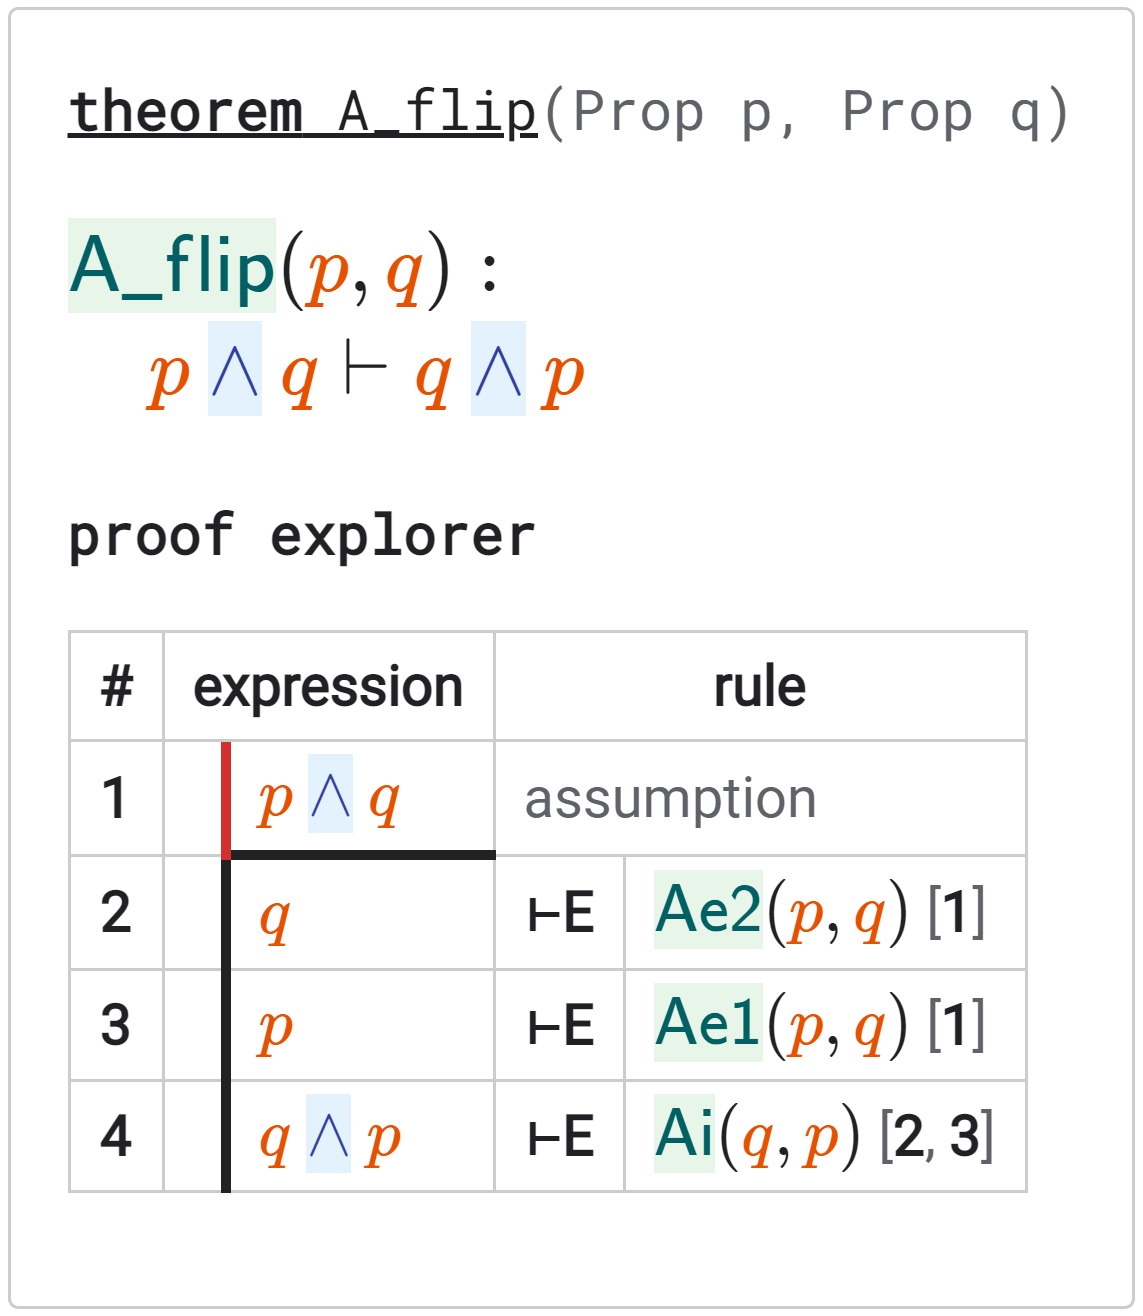
\includegraphics[scale=.18]{A_flip}
	\caption{\texttt{A\_flip}의 증명} \label{fig:Aflip}
\end{figure}

이름이 초록색으로 표시된 것은 증명이 \texttt{math-o-matic} 프로그램의 검증을 통과하였다는 뜻이다.

\section{현재의 형식 체계}

현재 \texttt{math-o-matic} 체계 상에서 만든 형식 체계는 Morse--Kelley 집합론을 기반으로 하여 이항관계, 함수, 자연수 집합 및 정수 집합에 관한 이야기를 할 수 있다.

\subsection{공리계}

현재 17개의 공리가 있으며, 명제논리를 위한 공리계는 예시~\ref{example:system}의 $\mathcal H_0$와 같다. 또 술어논리를 위한 공리는 두 개 뿐인데, 다음과 같다.
\begin{align*}
	\mathsf{Ui}&\coloneqq (f^{\mathsf{Predicate}})\mapsto (f\vdash\forall f), \\
	\mathsf{Ue}&\coloneqq (f^{\mathsf{Predicate}}, x^\Cls)\mapsto (\forall f\vdash f(x)).
\end{align*}
Morse--Kelley 집합론을 기반으로 하므로 $x$가 집합 타입 $\Set$이 아니라 클래스 타입 $\Cls$이다. $\forall$은 타입이 $\mathsf{Predicate}\to\Prop$인 무정의용어로 정의되는데, 이는 $(\forall x)(f(x))$를 $\forall(x\mapsto f(x))$로 변형한 것이다. 집합론을 위한 공리는 외연성 공리(axiom of extensionality)나 멱집합 공리 등이 있으며 Morse--Kelley 집합론의 공리들을 가져 온 것이다.

\subsection{증명된 정리들}

우리 체계에서 증명된 500개 가량의 정리 중에서 주목할 만한 것들은 다음과 같다.

\begin{itemize}
	\item $1+1=2$ (\textsf{one\_plus\_one\_is\_two}).
	\item 수학적 귀납법 (\textsf{induce}).
	\item Cantor의 정리 (\textsf{cantor}).
	\item Schr\"oder--Bernstein 정리 (\textsf{schroeder\_bernstein}).
\end{itemize}

\subsection{완전성}

우리의 체계는 페아노 공리계의 공리들을 증명할 수 있으므로 G\"odel의 불완전성 정리에 의하여 일관적이면서 완전할 수 없다.

\section{결론 및 향후 연구}

공리계간의 isomorphism에 관해 생각해볼수잇을듯하다.

\bibliography{bib}

\end{document}